\documentclass{beamer}
\usetheme{default}
\usepackage{amssymb}

\usepackage[utf8]{inputenc}

\usepackage{textcomp}
\usepackage[mathletters]{ucs}
\begin{document}

% --- Title slide ---

\title{Rating Systems (..in Gaming)}
\subtitle{Ratingsysteme verstehen, nachbauen und misbrauchen}
\author{Yannik Schmidt\vspace{-.3cm}}
\institute{Lightningtalks @FAU}
\date{}

\begin{frame}
\titlepage
\vspace{-1.2cm}
\begin{center}
\end{center}
\end{frame}

% --- Main content ---

\begin{frame}{Rating Systems - Basics}
\begin{figure}[H]
\centering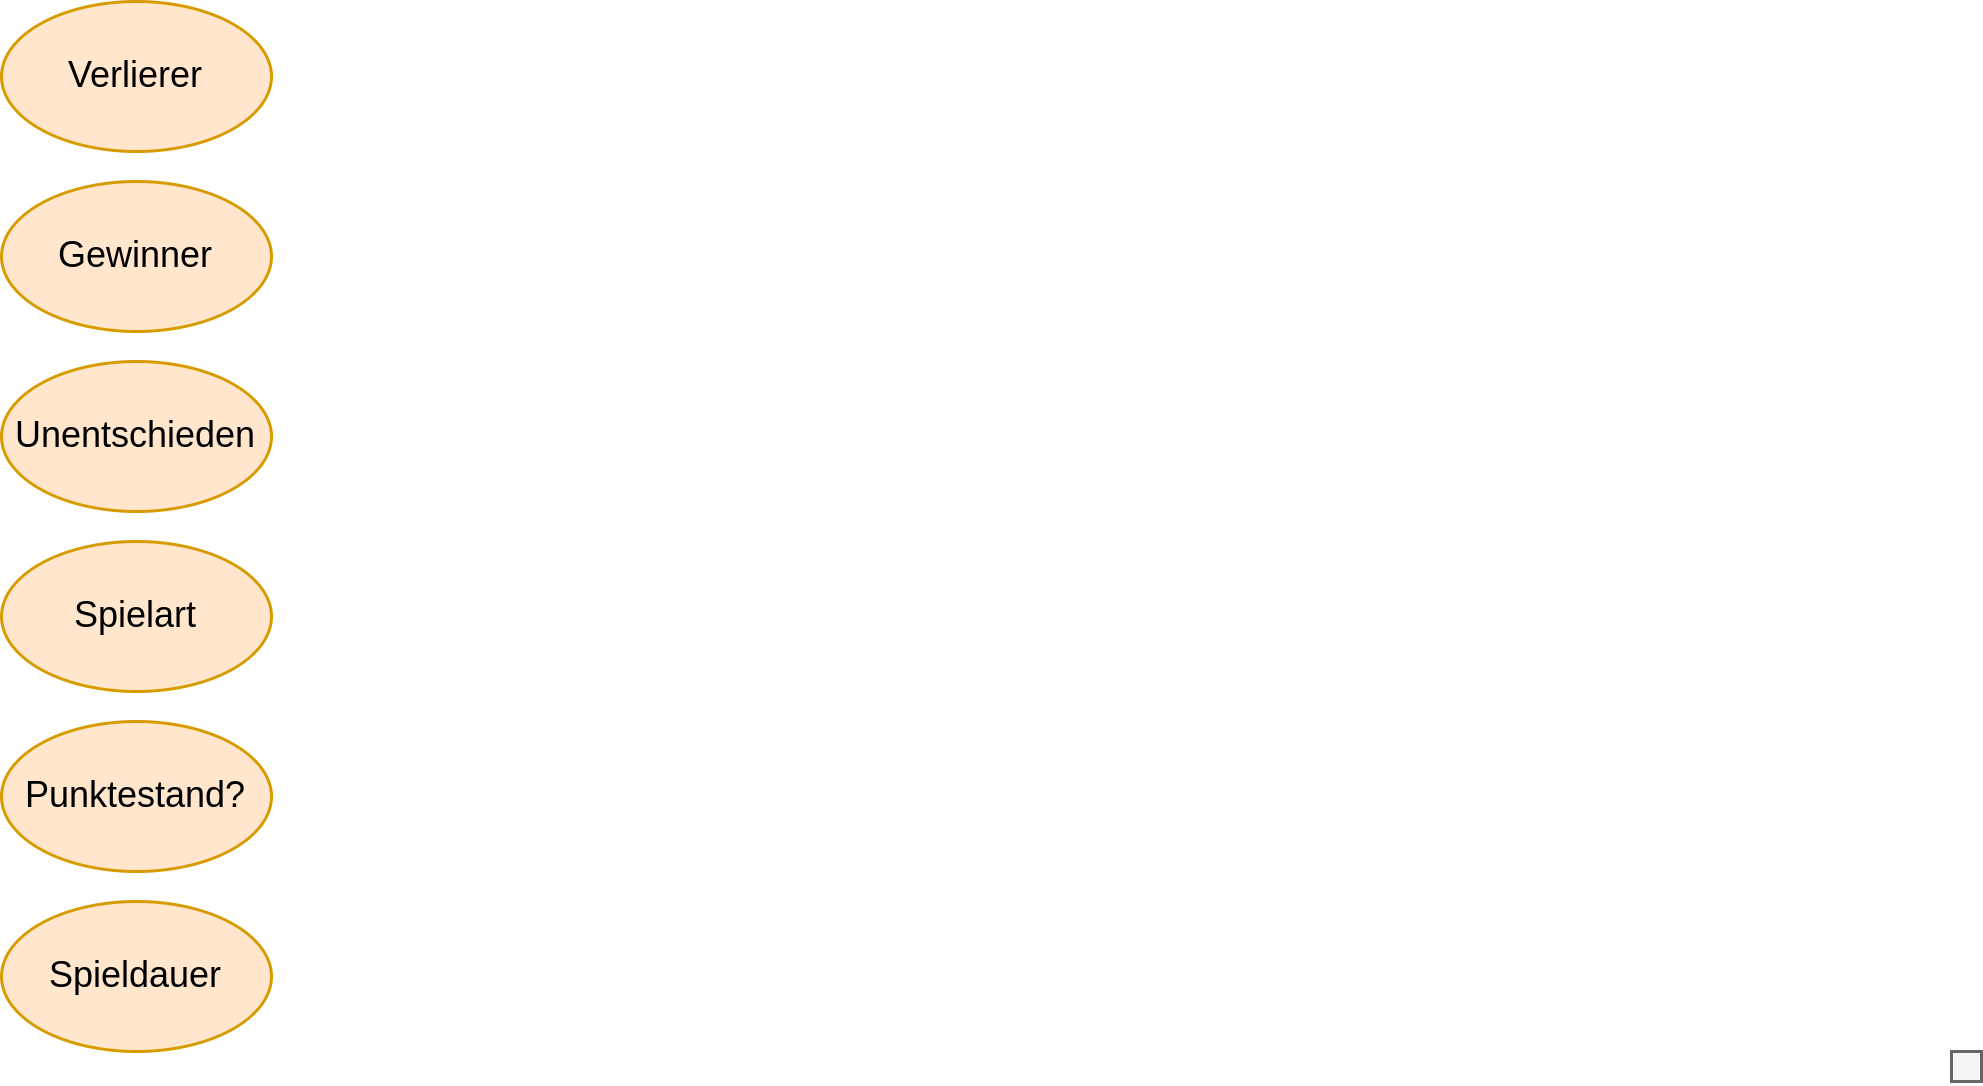
\includegraphics[width=10cm]{ratingsystem_basics_1.drawio.png}
\end{figure}
\end{frame}

\begin{frame}{Rating Systems - Basics}
\begin{figure}[H]
\centering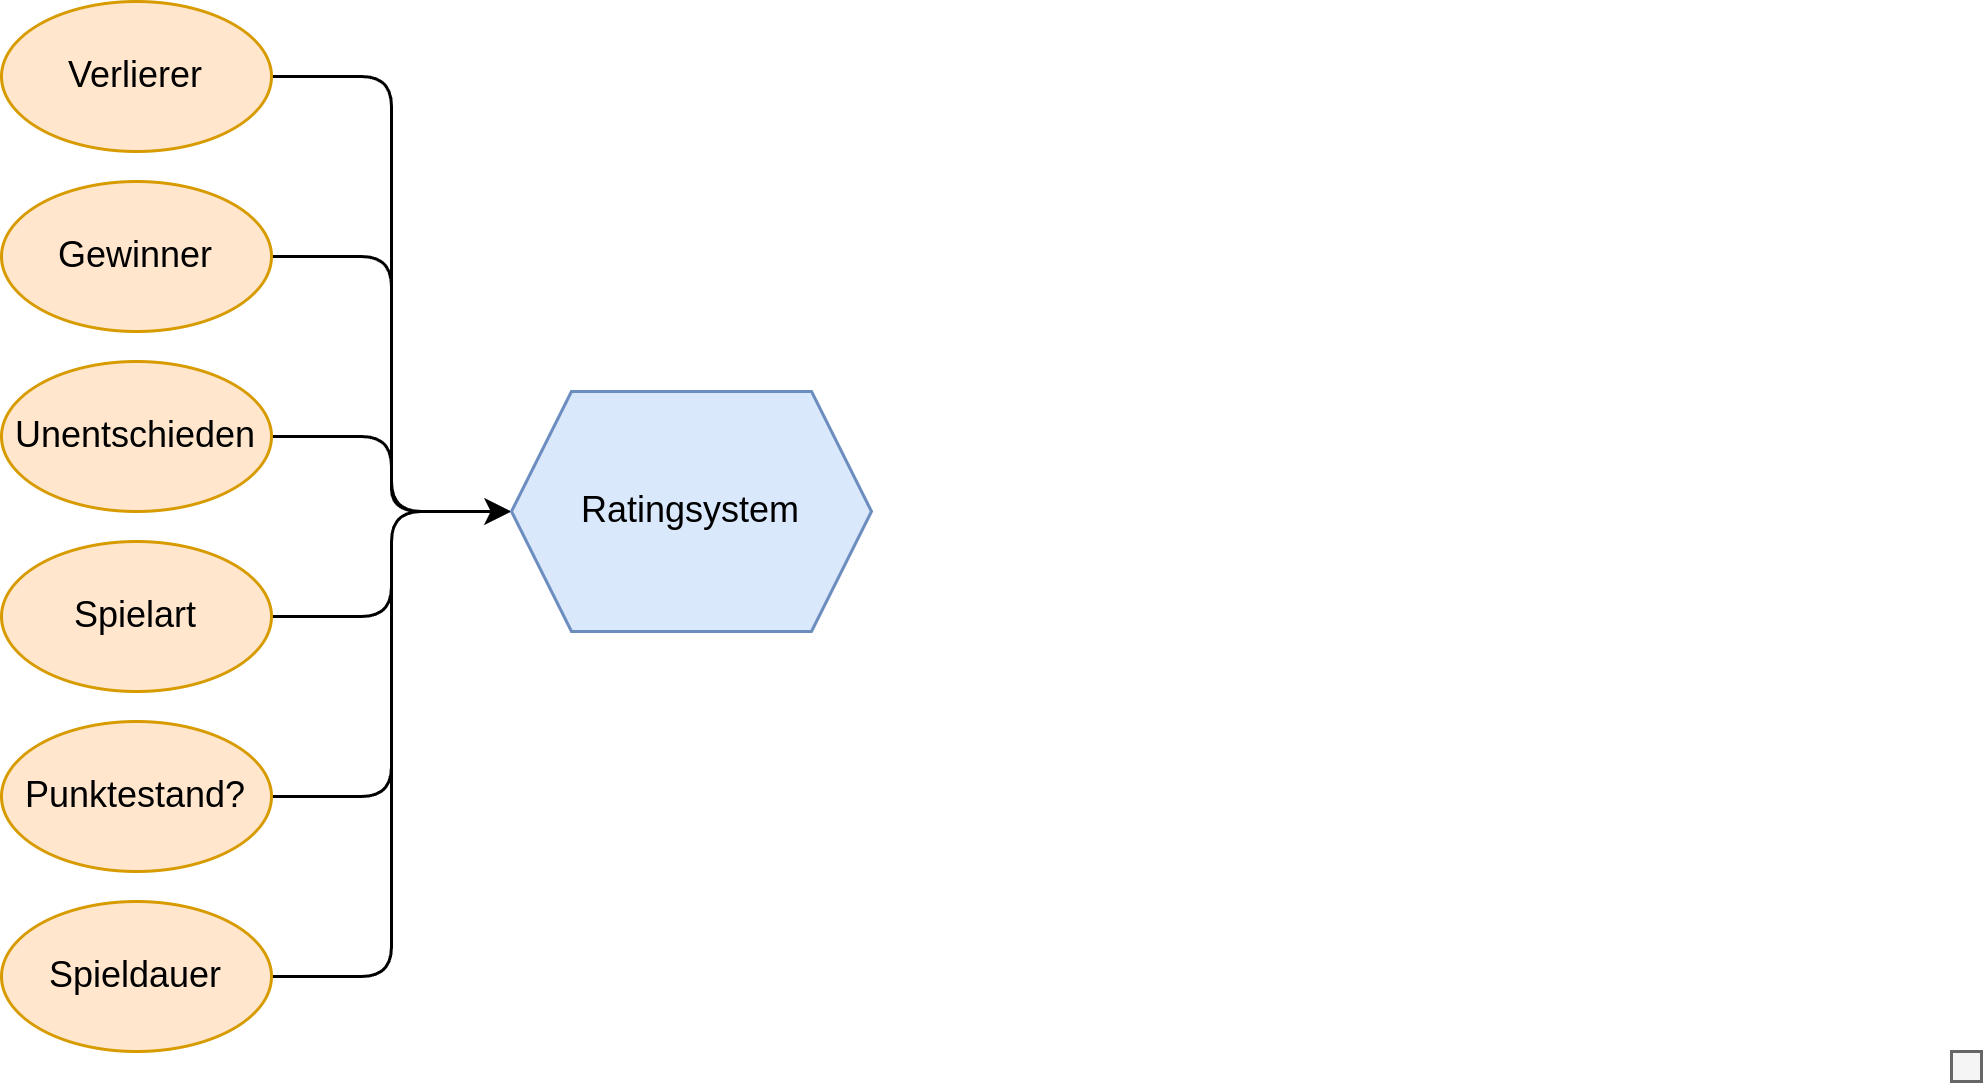
\includegraphics[width=10cm]{ratingsystem_basics_3.drawio.png}
\end{figure}
\end{frame}

\begin{frame}{Rating Systems - Basics}
\begin{figure}[H]
\centering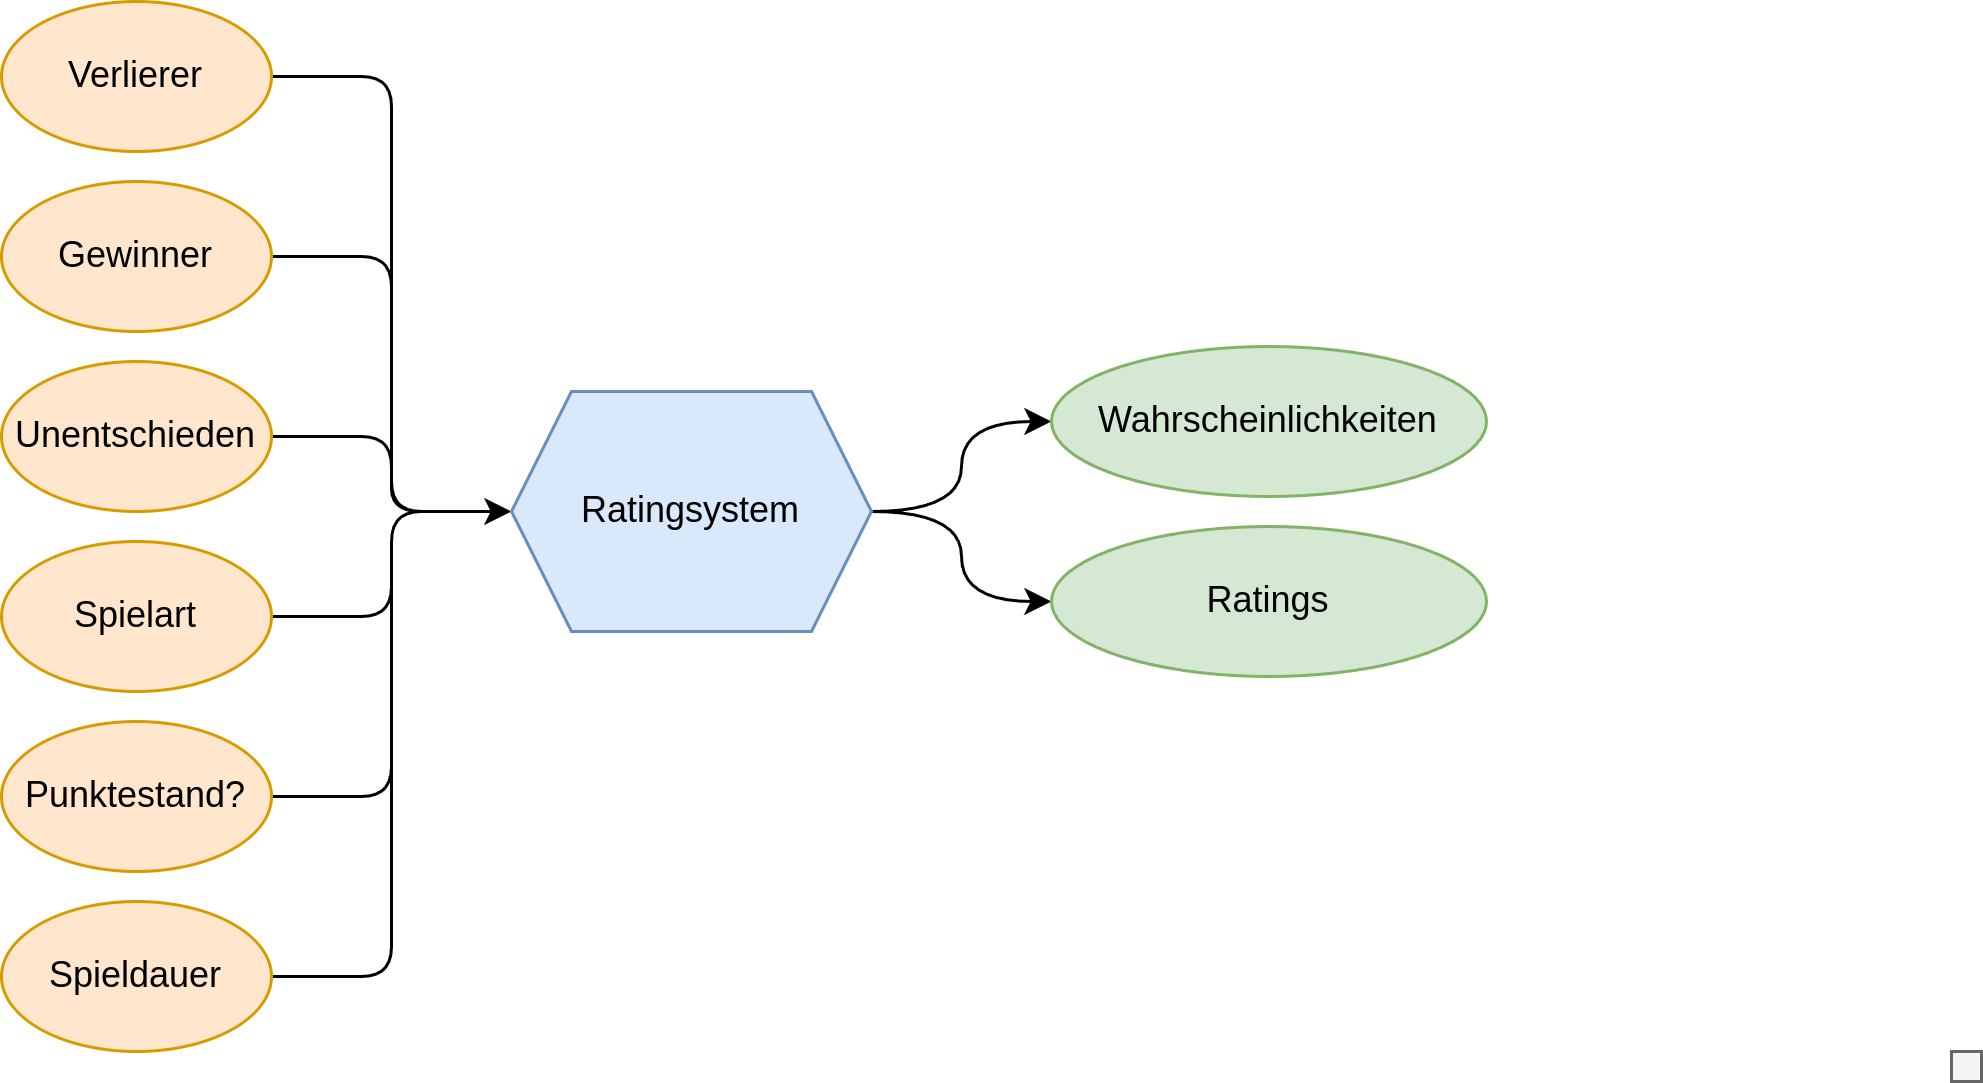
\includegraphics[width=10cm]{ratingsystem_basics_4.drawio.png}
\end{figure}
\end{frame}

\begin{frame}{Rating Systems - Basics}
\begin{figure}[H]
\centering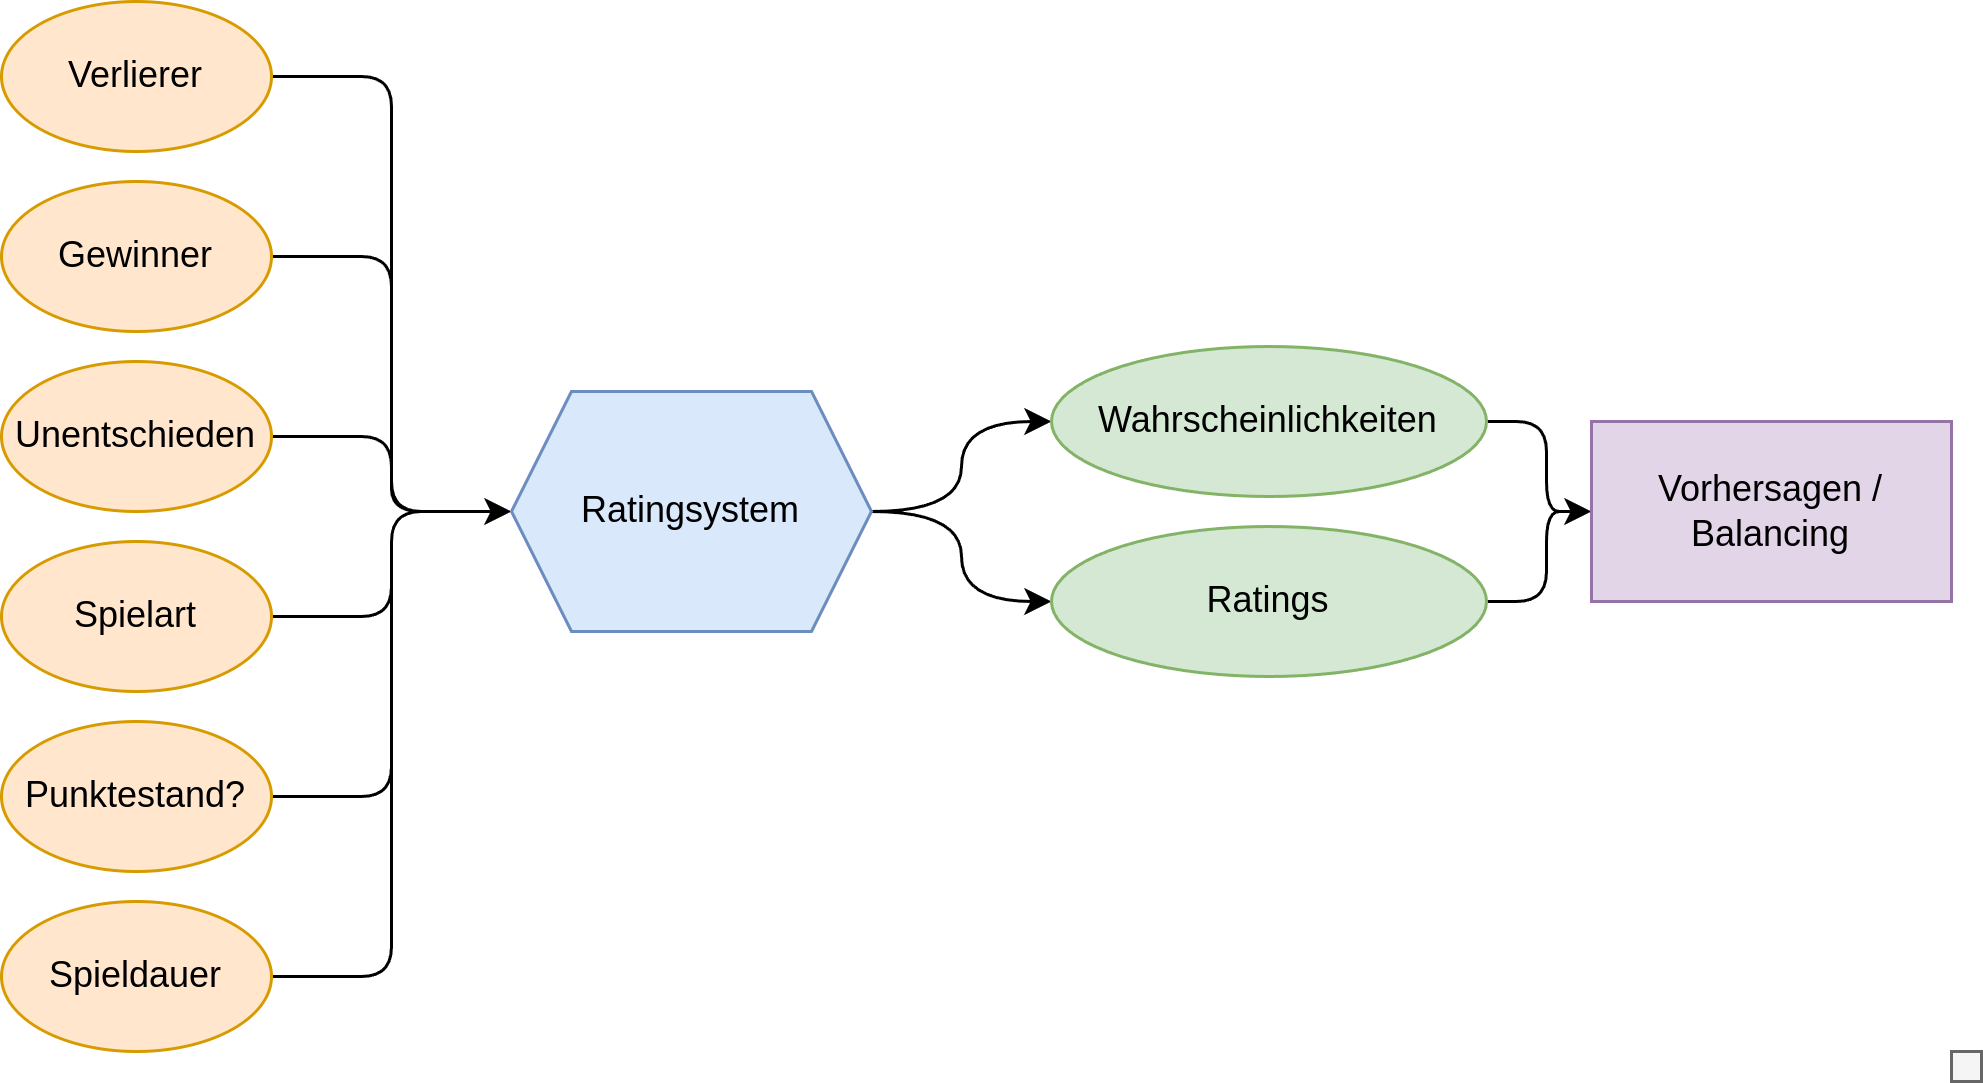
\includegraphics[width=10cm]{ratingsystem_basics_5.drawio.png}
\end{figure}
\end{frame}

\begin{frame}{Rating Systems - Siegesrate}
\begin{itemize}
\item 10 Spiele gespielt
\item Spieler A: 3 Siege
\item Spieler B: 7 Siege
\item Gewinnwahrscheinlichkeit Spieler B: 70\%
\end{itemize}
\end{frame}

\begin{frame}{Rating Systems - Realität}
\centering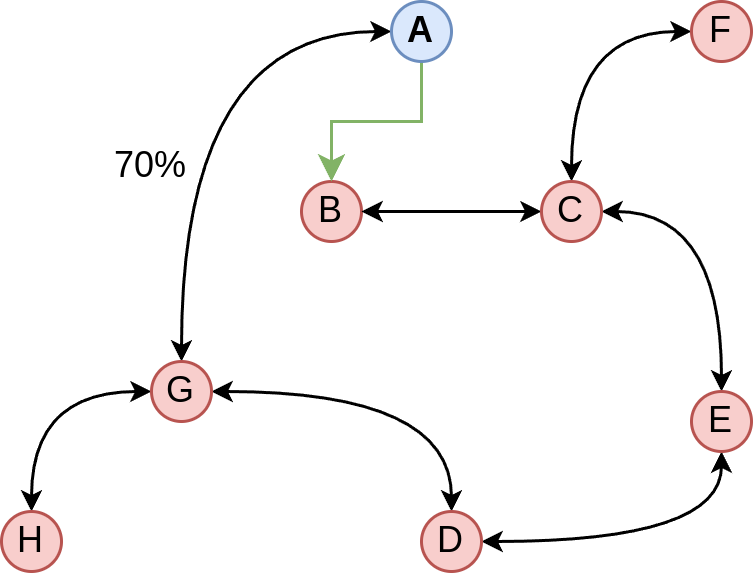
\includegraphics[width=8cm]{player_graph_1.drawio.png}
\end{frame}

\begin{frame}{Rating Systems - Realität}
\centering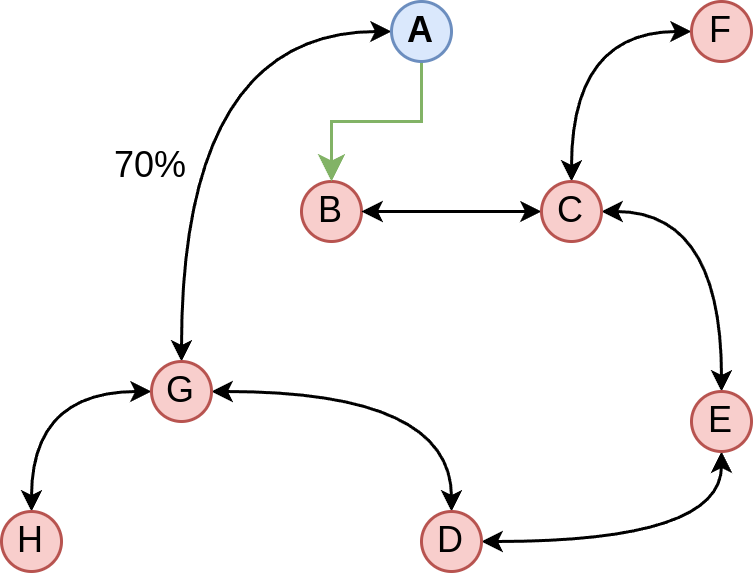
\includegraphics[width=8cm]{player_graph_1_number_1.drawio.png}
\end{frame}

\begin{frame}{Rating Systems - Realität}
\centering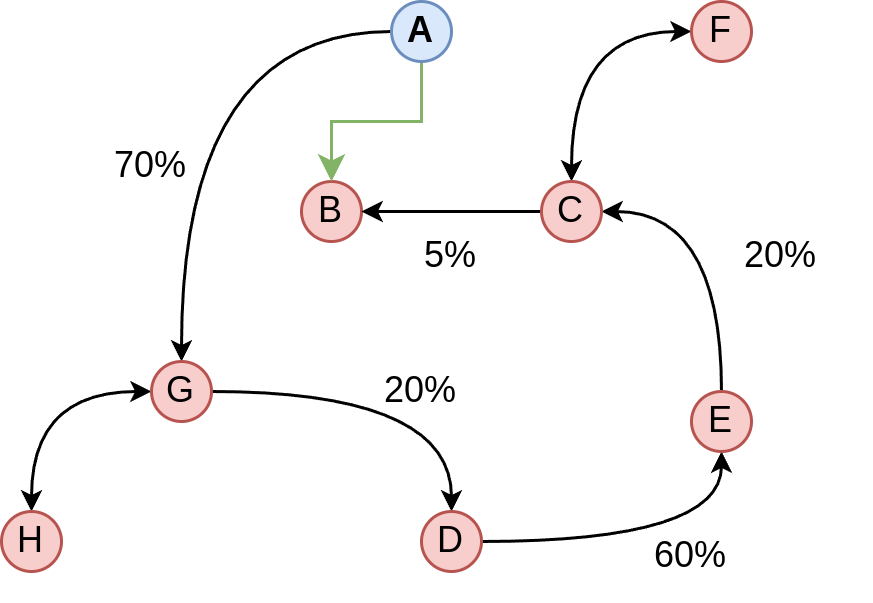
\includegraphics[width=8cm]{player_graph_1_number_all.drawio.png}
\begin{itemize}
\vspace{0.5cm}
\pause
\item $P(A>B) \approx  P(G>D) \times P(D>E) \times P(E>C) \times P(C>B)$\\
\vspace{2mm}
$\color{red}{\approx 1.74\%}$
\end{itemize}
\end{frame}

\begin{frame}{Ein einfacher Rating-Graph - Probleme}
\begin{itemize}

\item Mehrere Pfade sind möglich
\pause
\item Wie werden mehrere Pfade gewichtet?
\pause
\item Aufwand alle Pfade zu finden potenziell $O(n^3)$
\pause
\item Speicheraufwand für Kanten
\pause
\item N gegen N ???
\pause
\item Resilienz gegen adverse Echtwelt-Situationen
\end{itemize}
\end{frame}


\begin{frame}{Ratingsysteme - Resilienz und Stabilität}
\begin{itemize}
\item Was macht ein Ratingsystem "gut" ?
\item Mit welchen Problemen muss ein Ratingsystem klarkommen?
\end{itemize}
\end{frame}

\begin{frame}{Ratingsysteme - Resilienz und Stabilität}
\framesubtitle{Unsichere Verbinndungen und Outlier}
\centering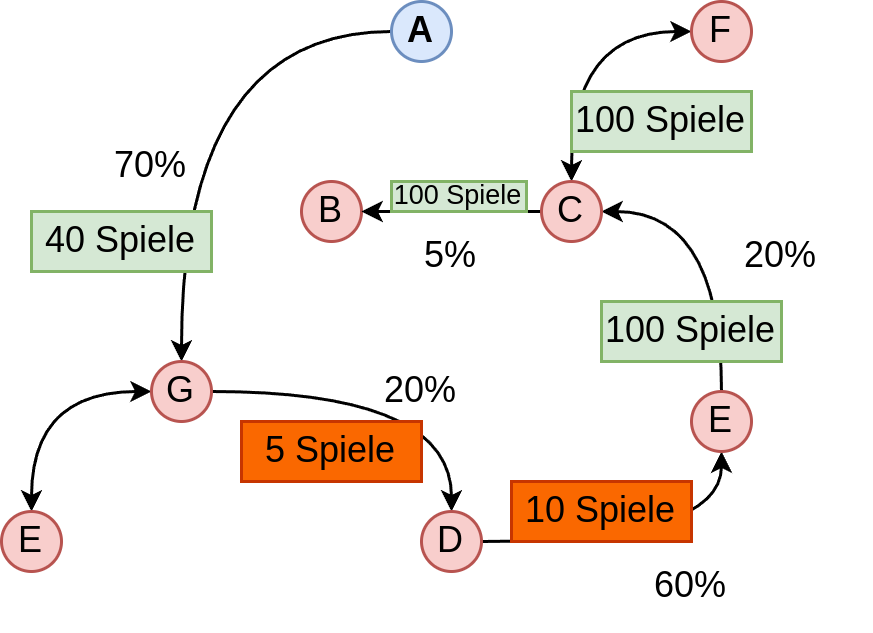
\includegraphics[width=10cm]{player_graph_1_number_unsicherheit.drawio.png}
\end{frame}

\begin{frame}{Ratingsysteme - Resilienz und Stabilität}
\framesubtitle{Veränderung}
\centering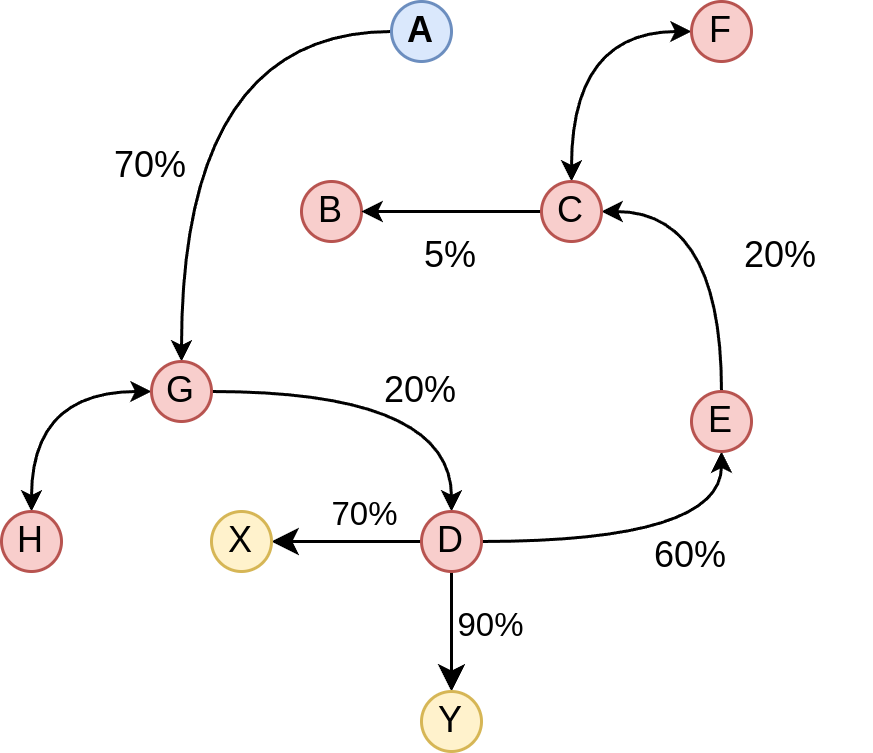
\includegraphics[width=8cm]{player_graph_1_number_change.drawio.png}
\end{frame}

\begin{frame}{Ratingsysteme - ELO}
\centering
\begin{equation}
\notag
\displaystyle E = \frac{1}{1 + 10^{\frac{R_{\text{A}} - R_{\text{B}}}{K}}}
\end{equation}
\vspace{1.8cm}
\end{frame}

\begin{frame}{Ratingsysteme - ELO}
\centering
\begin{equation}
\notag
\displaystyle E = \frac{1}{1 + 10^{\frac{R_{\text{A}} - R_{\text{B}}}{\color{red}{400}}}}
\end{equation}
\vspace{1cm}
\pause
\begin{equation}
\notag
\displaystyle \Delta R_{\text{player}} = K \times (1 - E)
\end{equation}
\end{frame}

\begin{frame}{Ratingsysteme - ELO}
\begin{table}[h!]
\centering
\begin{tabular}{|c|c|c|}
\hline
\textbf{Rating Unterschied} & \textbf{Gewinnchance}\\ \hline
-500 & \color{red!95} 5.3 \% \\ \hline
-400 & \color{red!85} 9.1 \% \\ \hline
-300 & \color{red!75} 15.1 \% \\ \hline
-200 & \color{red!65} 24.0 \% \\ \hline
-100 & \color{red!60} 36.0 \% \\ \hline
-50  & \color{gray!90} 42.9 \% \\ \hline
0    & \color{gray!90} 50.0 \% \\ \hline
50   & \color{gray!90} 57.1 \% \\ \hline
100  & \color{green!60} 64.0 \% \\ \hline
200  & \color{green!65} 76.0 \% \\ \hline
300  & \color{green!75} 84.9 \% \\ \hline
400  & \color{green!85} 90.9 \% \\ \hline
500  & \color{green!95} 94.7 \% \\ \hline
\end{tabular}
\end{table}
\end{frame}

\begin{frame}{Ratingsysteme - ELO}
\begin{itemize}
\item ..konvergiert langsam
\item ..performt schlecht in Edge-Cases
\item ..hat kein Konzept eines Unentschieden
\item ..in Reinform nur 1v1
\item ..neigt zu Inflation
\item ..keine Abbildung von "Tagesform"/Varianz
\end{itemize}
\end{frame}

% und natürlich wenn ein System nicht gut funktioniert beginnt das "basteln"
\begin{frame}{Ratingsysteme - ELO}
\begin{itemize}
\item Provisorische Ratings
\item Manuelle Anpassungen
\item Variabler K-Faktor
\item Durchschnitts Ratings für N vs. N
\end{itemize}
\end{frame}

% aber, aber selbst mit allen diesen Nachteilen, sollte allen klar sein, was wir nun gefixt haben, jeder spieler hat nur eine einzelne Zahl die direkt verglichen werden kann und wenn neue Information über einen spieler dazu kommen, dann werden diese auch in dieser Zahl repräsentiert sind nicht verloren wenn wir einem Anderen Pfad folgen
% worüber das natürlich nicht hinwegtäuschen sollte, ist dass einige der unterliegenden Probleme immer noch existieren, schwachen verbinndungen zwischen clustern (z.B. zwischen Region Servern in online spielen) können zu drift zwischen verschiedenen stark verbundenen gruppen führen und wir haben jetzt auf eine einzige Dimension reduziert, aber ist das wirklich was wir wollen, ein spieler spielt nicht auf "einem" level, dieser level wird jedes einzelnes spiel varieren, wegen tagesform, tageszeit, individuelle matchup unterschiede was auch immer, und genau diese Information haben wir hier jetzt verloren und damit sind 
\begin{frame}{Ratingsysteme - ELO Vorteil}
\centering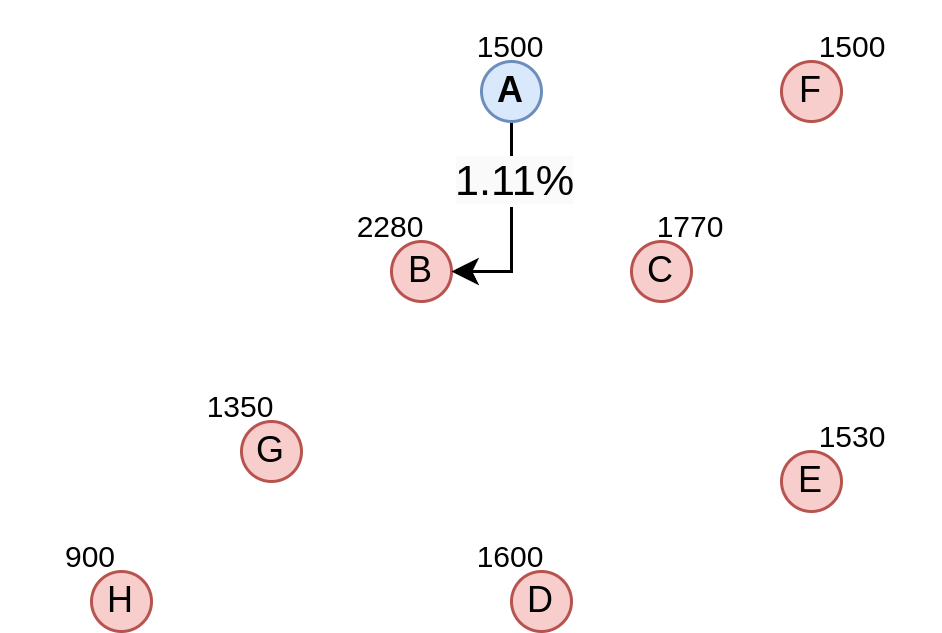
\includegraphics[width=8cm]{elo_graph.drawio.png}
\end{frame}

%
\begin{frame}{Ratingsyteme - Trueskill}
\huge ...ist ein Microsoft Trademark

\vspace{3cm}
\end{frame}

%
\begin{frame}{Ratingsyteme - Openskill}
\huge ...ist kein Microsoft Trademark\\
\vspace{3cm}
\small *Rechtsstreitigkeiten vermeidet man am besten bevor sie passieren.
\end{frame}

% die Idee hinter Trueskill bzw. Openskill, ist dass die performance eines Aktörs, welches ein rating am Ende wiederspiegelt, tatsächlich selbst eine Wahrscheinlichkeitsverteilung um einen mittelwert ist, daher werden Ratings nicht als zahl sonder mit sigma und mu, also einer Gauß-Verteilung angeben
\begin{frame}{Ratingsyteme - Openskill}
\centering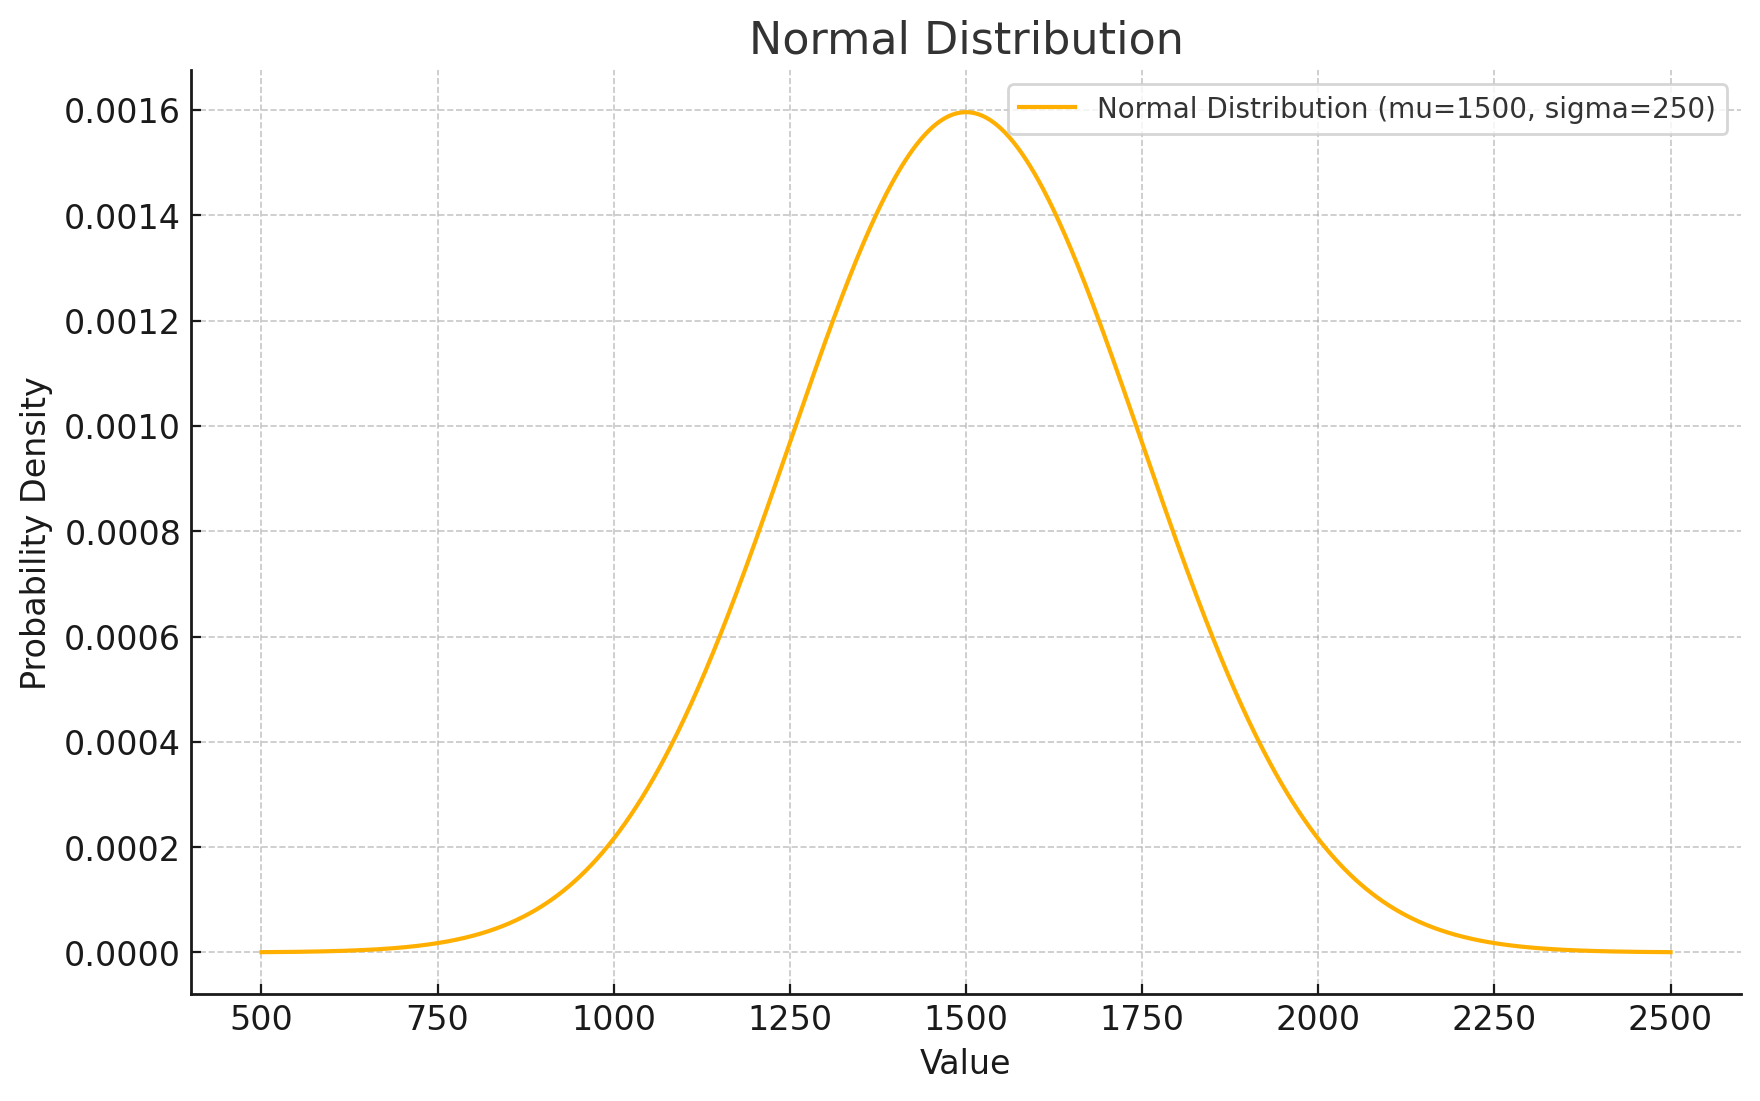
\includegraphics[width=10cm]{gauss.png}
\end{frame}

% und wenn wir dann zwei spieler haben, und sagen wir mal der zweite spieler hat eine engere wahrscheinlichkeits verteilung und ein höheres rating, dann können wir sehr natürlich daraus ableiten was die wahrscheinlichkeit ist, dass spieler Spieler A besser als spieler B ist
% openskill ist noch etwas mehr als das, für alle die hier schon etwas tief drin sind, was hoffentlich nicht so viele sind, denn die haben sich bisher wahrscheinlich etwas gelangweilt
\begin{frame}{Ratingsyteme - Openskill}
\centering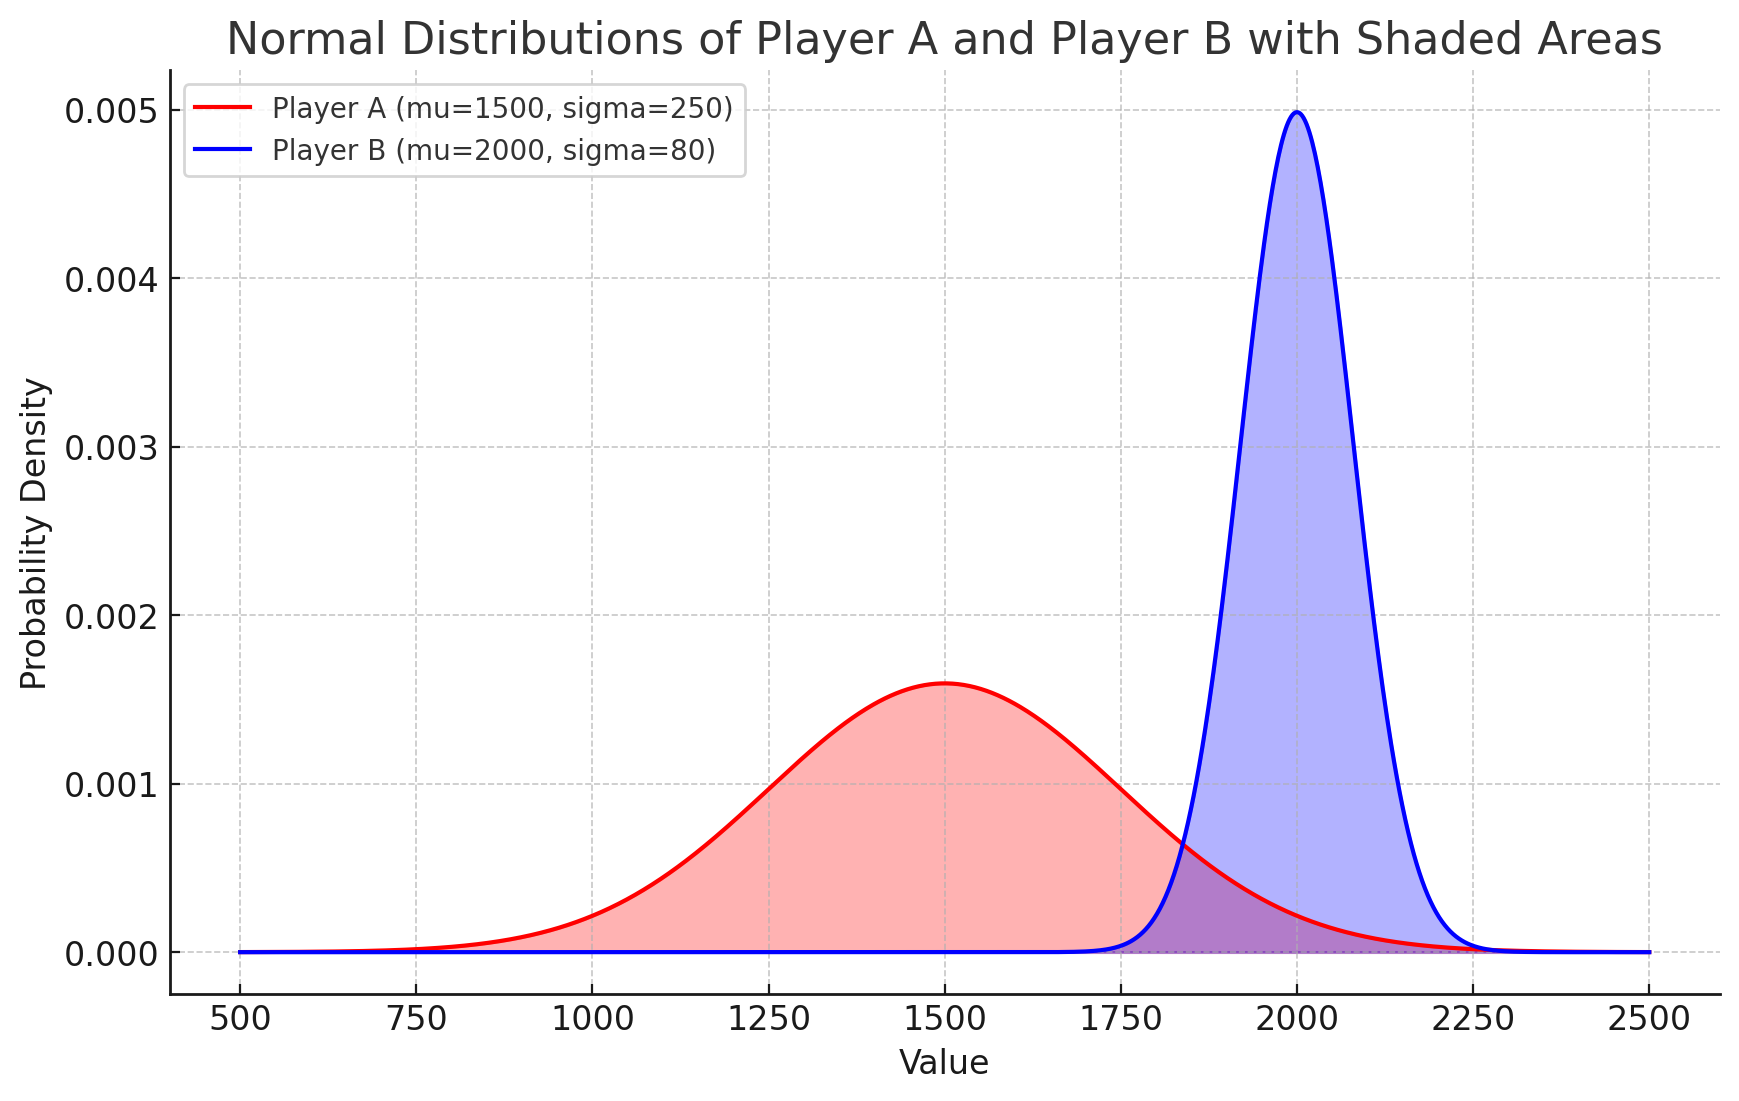
\includegraphics[width=10cm]{gauss_2.png}
\pause
$P(A > B) = \Phi\left(\frac{\mu_A - \mu_B}{\sqrt{\sigma_A^2 + \sigma_B^2}}\right) \approx  2.84\%$
\end{frame}

% die Eckpunkte sind
% und die Konvergenzgeschwindigkeit des Systems ist am Ende nichts anderes als ein Ausdruck den erwarteten Einfluss von Zufall auf unseren Ausgang unseres Spiel hat, wenn wir ein spiel mit viel würfel haben brauchen wir einen höheres Tau als bei einem Spiel das nahezu ausschließlich auf Skill besteht ein sehr niedriges tau=0.01
\begin{frame}{Openskill - Features}
\begin{itemize}
\item Teamratings können als Gauss-Summe abgebildet werden
\item Spieler mit niedriger Standardabweichung haben mehr Einfluss
\item Parameter $\tau$ für Konvergenzgeschwindigkeit
\item Ein \textit{weight}-Parameter für Spieler-Einfluss im Team
\end{itemize}
\end{frame}

% ich habe vor einigen jahren begonnen an einem Rating system für ein Spiel names insurgency zu schreiben, und als ich das begonnen habe kam ich von Leauge of Legends und wusste was das Rating system dort für ein clusterfuck sein kann und dachte das wird der Rating system Endgegener
\begin{frame}{Ratingsyteme - Insurgency}
\begin{itemize}
\item 8v8 bis 16v16
\pause
\item öffentliche Server, oft Spiele mit $>$50\% Spielern unter 3 Spielen
\pause
\item Join/Leaves während des Spiels, Teamwechsel möglich
\pause
\item asymmetrische Karten (Angriff und Verteidigung)
\end{itemize}
\end{frame}

% als ups keine guten vorrausstzungen also gut, was sind unsere Informationsdimensionen,
% außerdem bekommen wir die daten nur in form von events
\begin{frame}{Ratingsyteme - Insurgency Basis-Informationen}
\begin{itemize}
\item Karte geladen (MAP)
\item Spielstart Event (START)
\item Join Event (JOIN)
\item Leave Event (LEAVE)
\item Teamwechsel Event (CHANGE)
\item Spielende Event (END)
\end{itemize}
\end{frame}

% ok diese Informationen bringen wir jetzt in eine form, dass wir sie verwenden können und volia
\begin{frame}{Ratingsyteme - Abgeleitete Informationen}
\begin{itemize}
\item Spielstart - Spielende = Spieldauer
\item Join Event - (Change$|$End$|$Leave) = Spieldauer in Team
\item $[$ Spieldauer Team A - ( Spielerdauer Team B | 0 ) $]$ / Spieldauer = \textbf{Spielergewichtung}
\item Karte\_Defenders wird "Spieler" in Team A
\item Karte\_Attackers wird "Spieler" in Team B
\end{itemize}
\end{frame}

% nicht schlecht eh?
\begin{frame}{Rating Systems - Spiellänge}
\centering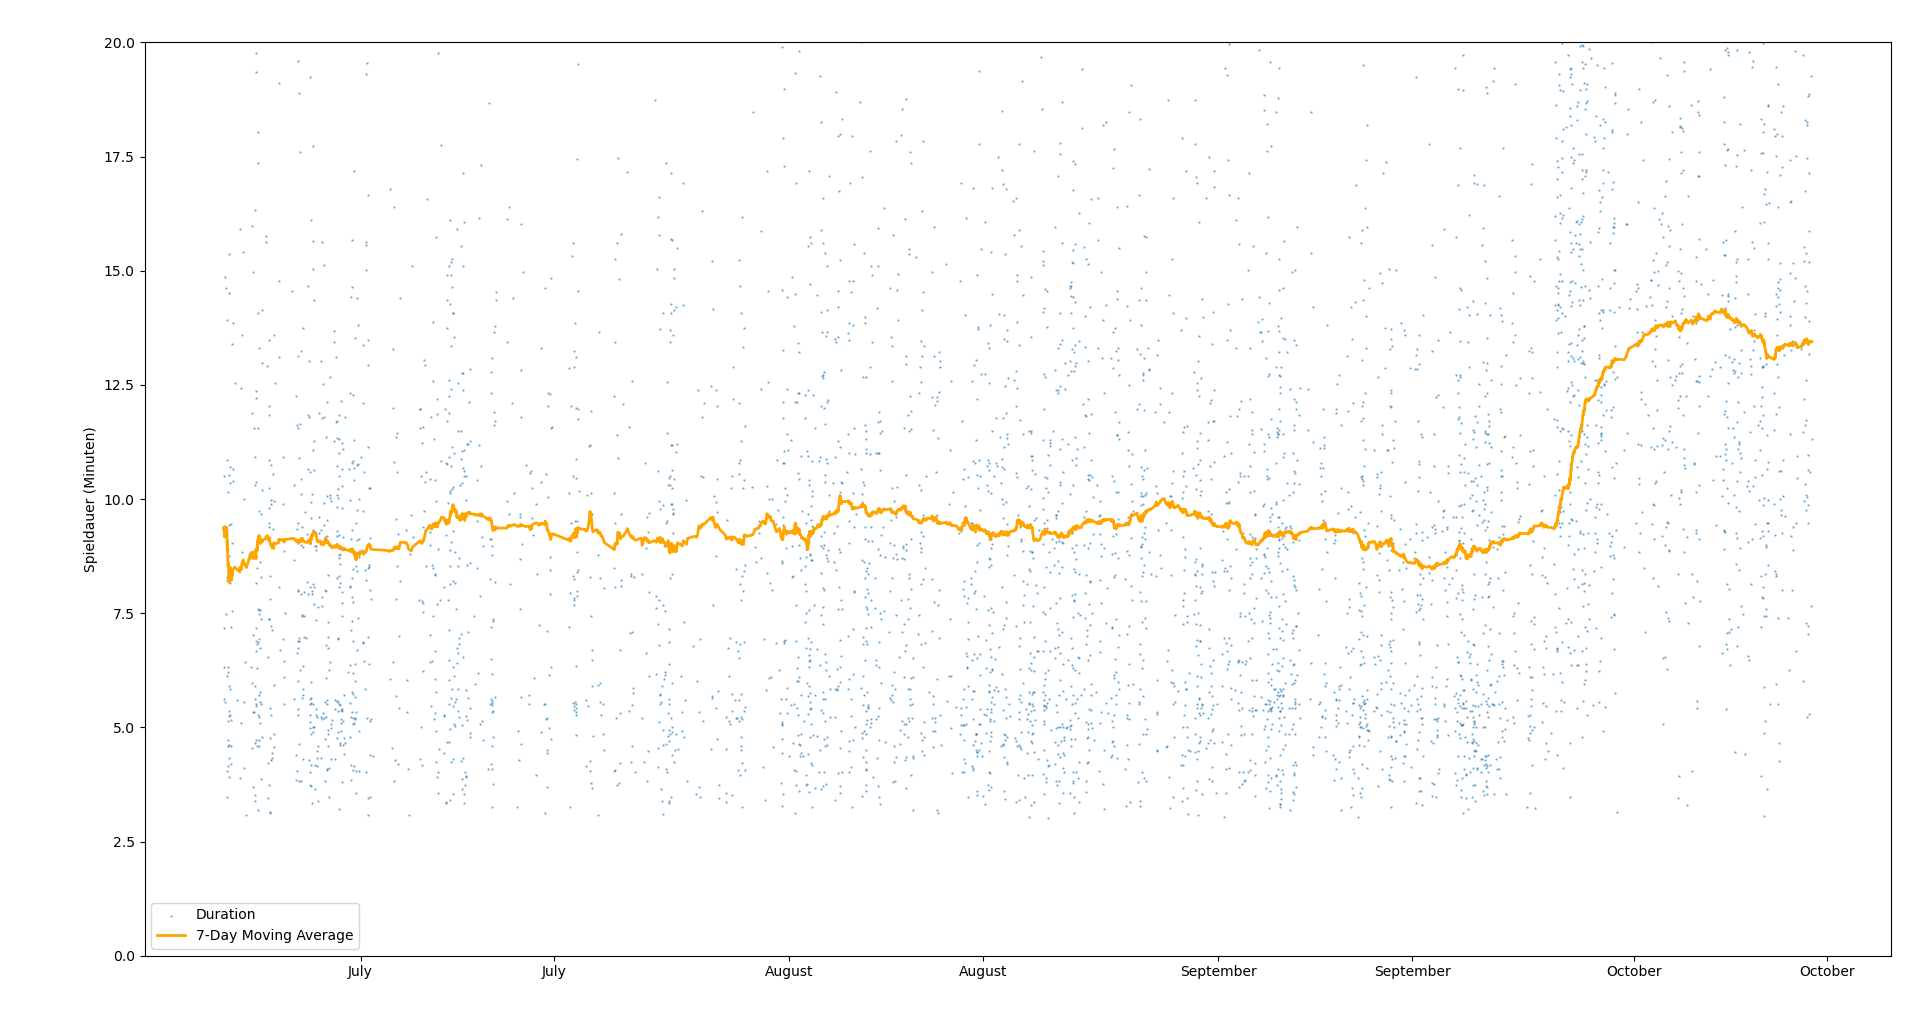
\includegraphics[width=11cm]{game_duration.png}
\end{frame}

% wie wärs mit player leave rate
\begin{frame}{Rating Systems - Spiellänge}
\centering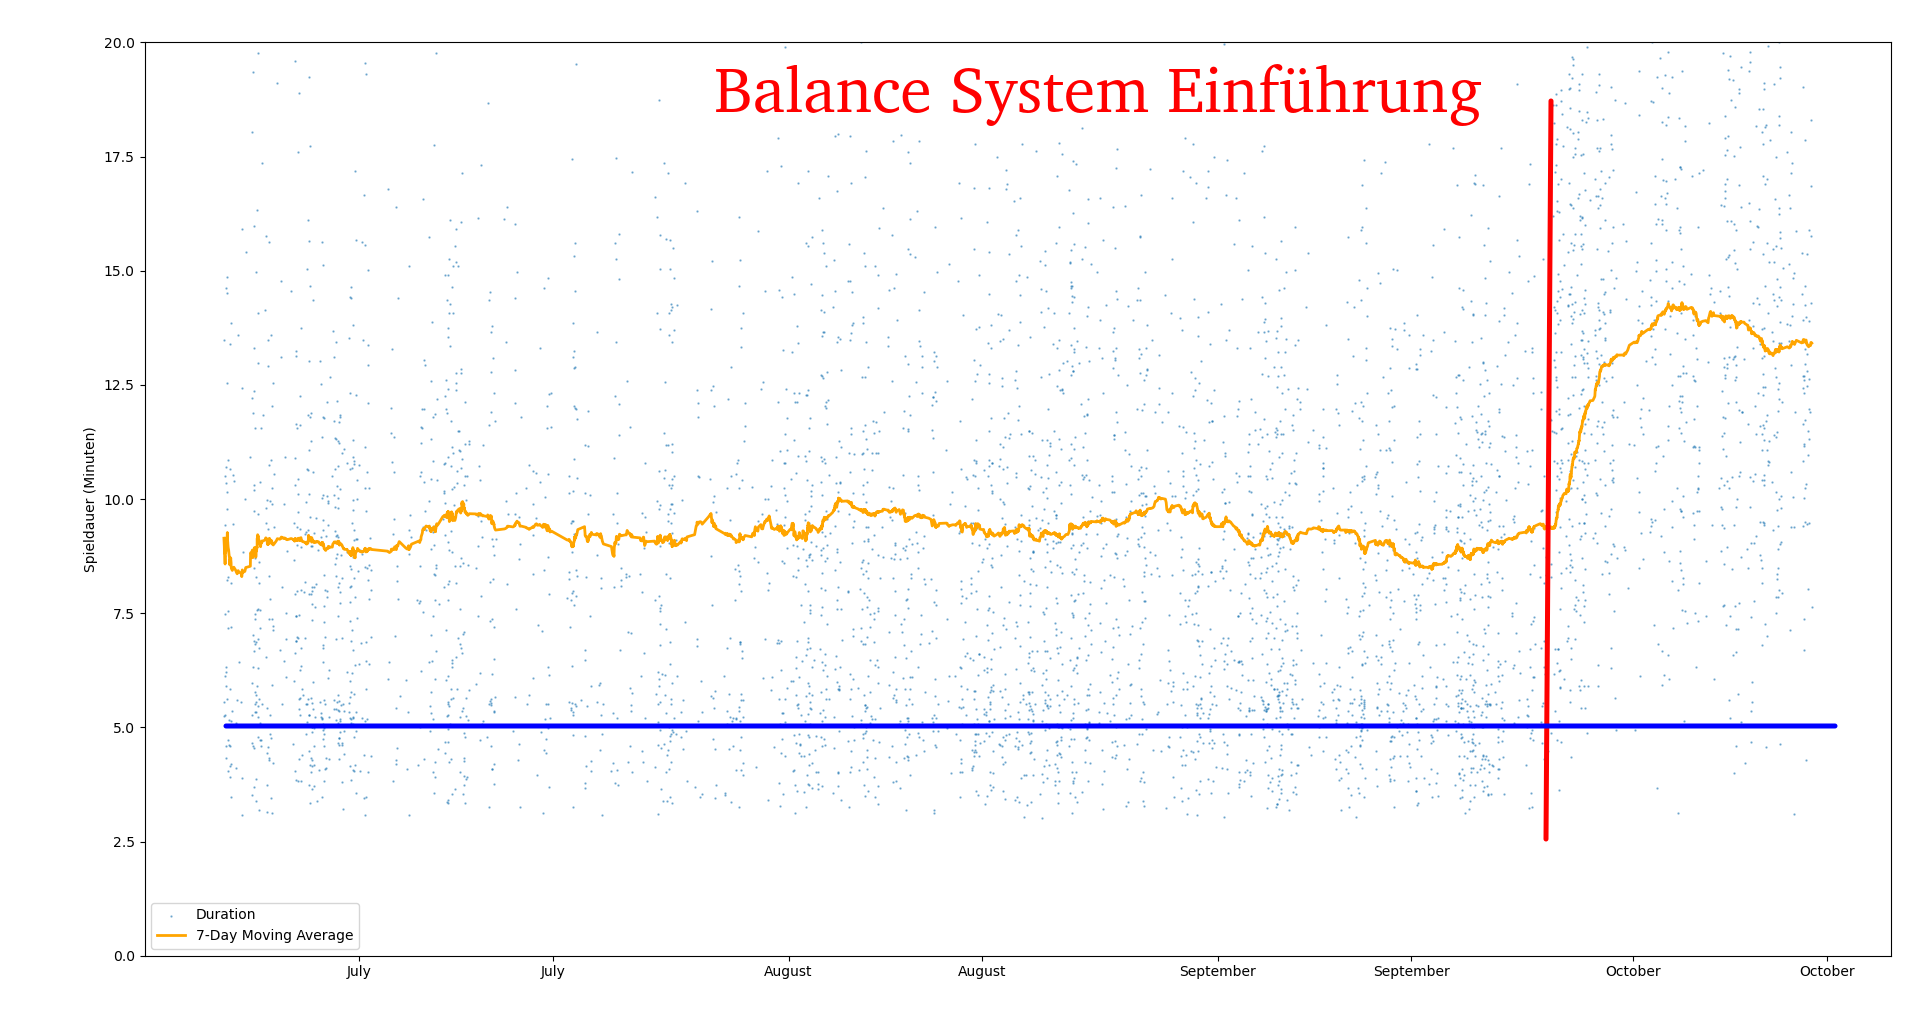
\includegraphics[width=11cm]{game_duration_edit.png}
\end{frame}

% aber ok jetzt sagt, ihr, cool, du hast jetzt hier daten über Jahre gesammelt, wie lang dauert es bis ein neuer Spieler richtig eingeranked ist, naja, 5 games, 5 games, wer von euch spielt LoL, wie viele games muss man da spielen damit man richtig eingeranked ist?
\begin{frame}{Rating Systems - Konvergenzzeit}
\centering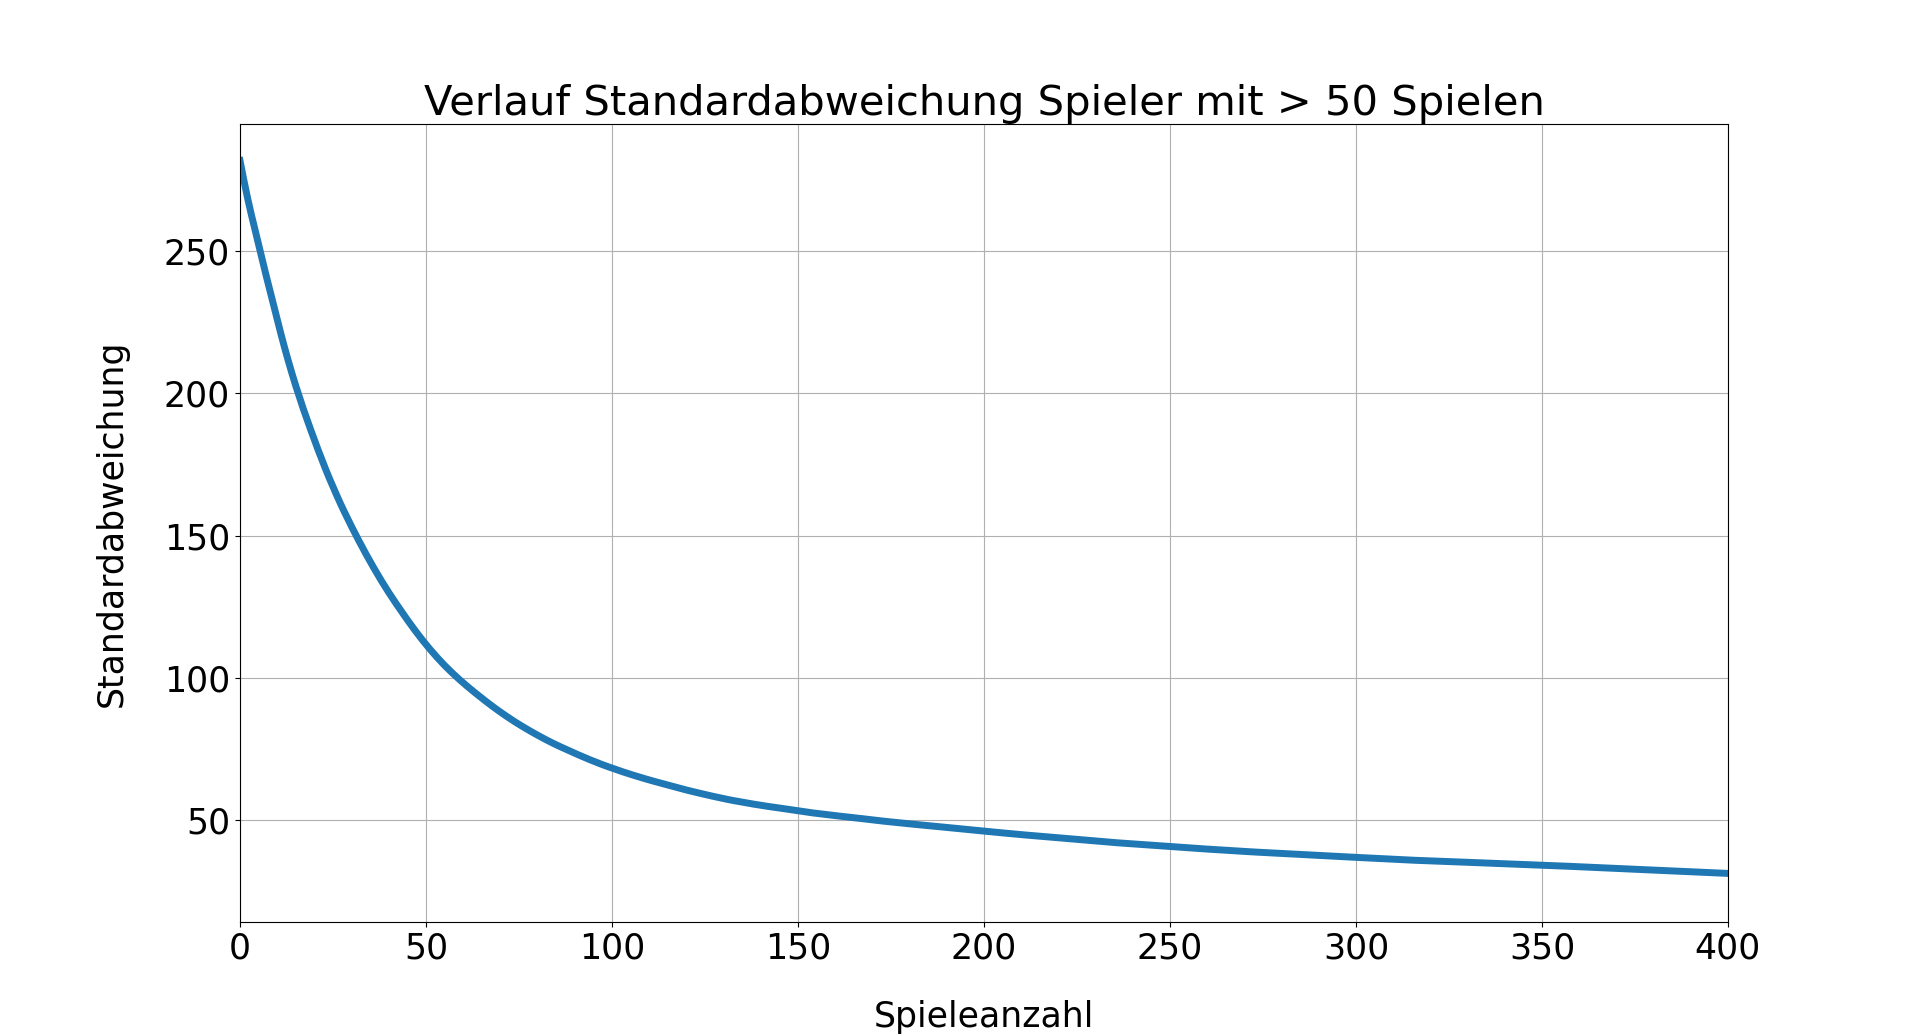
\includegraphics[width=11cm]{game_mu.png}
\end{frame}


% und ich schaue auf diese ergebnisse und denke mir, was im Name von Thomas Bayes treiben diese Idioten da, über Jahre lese ich im Devblog wie viel sie an ihrem Rating System gearbeitet wird, wie ist es möglich, dass die Konvergenzzeit eines Rating Systems trotzdem so hoch ist, in Leauge in FIFA in Valorant, was passiert hier sind die leute dort inkompetent
% es gibt gute spieler, aus den top Bereichen die 20-30, 50, 80 Spiele in Folge gewinnen, und glückwunsch, dass du gut bist, aber die realität ist
\begin{frame}{Rating Systems - "Shinanigans"}
\pause
\begin{itemize}
\item kein Rating System sollte 100+ Spiele zur Konvergenz brauchen
\item kein Balancing System sollte 10+ Spiele Gewinnserien zulassen
\pause
\item \textbf{..außer natürlich} \pause \textcolor{red}{..es ist eigentlich kein Balancing-System}
\end{itemize}
\end{frame}

% ja meine Herren, das ist ein Patent, von EA, welches beschreibt wie man Ratingsysteme in Multiplayer spielen benutzt um Microtransaktionsvolumen (also für alle die nicht wissen was das ist - Bezahlinhalte) zu erhöhen und spieler möglichst immer länger spielen lässt
% die meisten Modernen Rating systeme, in großen triple A online spielen, sind nicht desinged dafür, spiele zu balancen, sie sind dafür optimiert euch weiter spielen zu lassen
\begin{frame}{Rating Systems - "Shenanigans"}
\centering\includegraphics[width=11cm]{Patent.png}
\end{frame}

\begin{frame}{Fragen? Nächster Vortrag: DHCP!}
\begin{itemize}
\item \textbf{Implementierung}: github.com/FAUSheppy/skillbird
\footnote{\tiny FAU = \textbf{F}ucking \textbf{A}wesome \textbf{U}niversity}
\item \textbf{50 Seiten Openskill Mathe}: m.athq.de/ts.pdf
\item \textbf{Nächster Vortrag}: \textit{Funfacts über DHCP}
\item \textbf{Fragen}
\end{itemize}
\end{frame}

\end{document}